\section{Problema 1 - Puente sobre lava caliente}
\index{Problema 1 - Puente sobre lava caliente}



\subsection{Descripci\'on del problema a resolver}

Este problema nos plantea una situación en la cual un individuo desea atravesar un puente. Este puente está compuesto de una cantidad $n$ de tablones que pueden estar rotos o sanos. A su vez nuestro personaje puede saltar hasta una cantidad de $c$ de tablones por salto. Nuestro objetivo entonces es brindar una secuencia de saltos posibles que sea mínima en cantidad de saltos y que garanticen la integridad física del individuo impidiendo que pise tablones rotos.


Veamos algunos ejemplos para comprender mejor este enunciado:  

Instancia 1:

\begin{figure}[H]
\centering
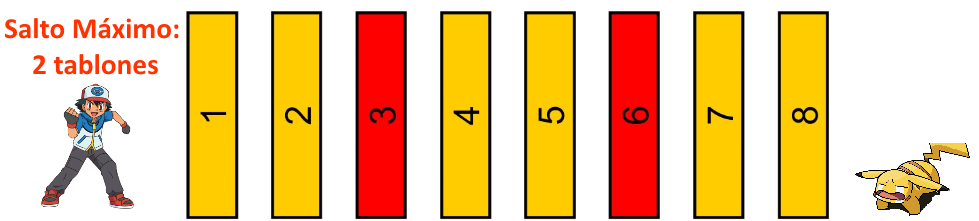
\includegraphics[scale=0.5]{ej1/tabl_1.png}
\end{figure}

En este caso la representación de la instancia que recibiremos como entrada será:

\begin{addmargin}[4em]{0em}
\textsf{8 2 0 0 1 0 0 1 0 0} \\
\textsf{0}
\end{addmargin}

En donde 8 es la cantidad total ($n$) de tablones, 2 ($c$) el salto máximo medido en tablones. Luego $n$ ceros o unos tales que $1$ representa un tablón roto y $0$ el estado contrario. El 0 final indica que termina la instancia.

La solución a esta instancia consta de 4 saltos. El primero al tablón 2, luego al 5, luego al 8 y finalmente fuera del puente. Esta solución la devolveremos de acuerdo al formato solicitado de la siguiente manera:

\begin{addmargin}[4em]{0em}
\textsf{4 2 5 8 11} \\
\end{addmargin}

Notemos 2 aspectos relevantes a la interpretación del problema en esta solución. En primer lugar, la cantidad $c$ de tablones máxima que se puede saltar implica que no puede haber más de $c$ tablones entre el tablón del cual se parte y el tablón al que se llega. De esta manera, por ejemplo, partiendo del tablón 2 con $c=2$ se podra llegar como máximo al tablón 5. 
Otro detalle importante consiste en notar que se empieza fuera del puente y se debe terminar fuera de él también. Podria verse como que existe un tablón $0$ del cual se parte y cualquier número mayor a $n$ en la salida indica que estamos fuera del tablón. Por este motivo, en este caso, el último valor de la salida es 11, que corresponde a realizar el salto máximo desde el tablón 1. 

Dicho esto veamos que para este caso sólo había una solución posible que minimiza los saltos y también que en cada salto el personaje saltarin termina en el tablón sano más lejano posible. Más adelante en este informe demostraremos que esta intuición efectivamente sirve para garantizar los mínimos saltos posibles, sin embargo, consideramos importante notarlo en estas instancias previas.

Analicemos otra instancia:

\begin{figure}[H]
\centering
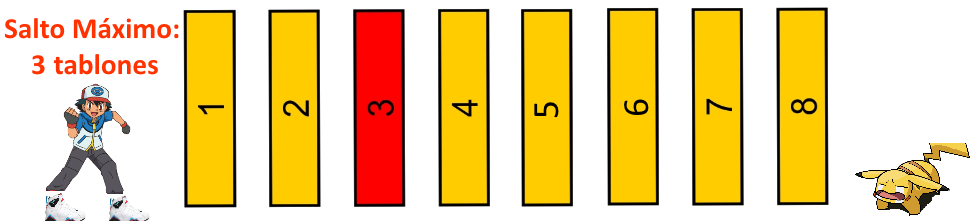
\includegraphics[scale=0.5]{ej1/tabl_3.png}
\end{figure}

En este caso la entrada recibida se verá asi: 

\begin{addmargin}[4em]{0em}
\textsf{8 3 0 0 1 0 0 0 0 0} \\
\textsf{0}
\end{addmargin}

Nuevamente tenemos 8 tablones pero ahora solo uno roto y podemos saltar de a 3. 

Veamos también la salida de nuestro algoritmo:

\begin{addmargin}[4em]{0em}
\textsf{3 4 8 12} \\
\end{addmargin}

Lo destacable de esta instancia es que permite varias soluciones. Si bien, como explicamos previamente, nuestro algoritmo siempre salta al tablón sano más lejano, una solución posible consite en saltar primero al tablón 4, luego al 7 y luego salir del puente, sin saltar más veces. Cualquier solución de saltos mínimos es permitida como salida de este problema.

Por último notemos la siguiente instancia

\begin{figure}[H]
\centering
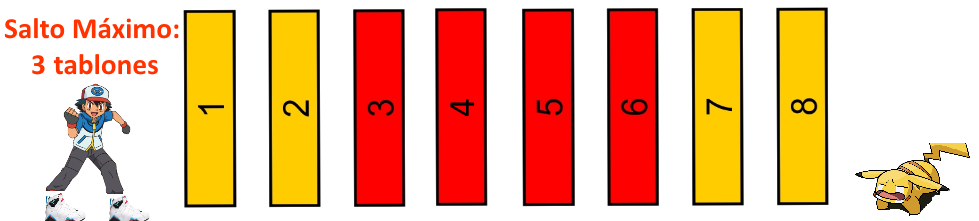
\includegraphics[scale=0.5]{ej1/tabl_2.png}
\end{figure}

Cuya entrada es: 
\begin{addmargin}[4em]{0em}
\textsf{8 3 0 0 1 1 1 1 0 0} \\
\textsf{0}
\end{addmargin}

La salida en este caso es:

\begin{addmargin}[4em]{0em}
\textsf{no} \\
\end{addmargin}

Este \textbf{no} indica que no hay solución para esta instancia, dato que puede obtenerse de la observación de la entrada, ya que tenemos más tablones rotos consecutivos de los que podemos saltar en un salto.

Habiendo recorrido entonces un espectro amplio de casos posibles, en la siguiente sección describiremos más detalladamente las ideas involucradas(con su demostración) en la solución de este problema.

\subsection{Ideas desarrolladas para la resoluci\'on}

Como ya hemos expresado previamente, hay una premisa que pareciera guiarnos hacia la solución de este problema y es la idea de que, para minimizar la cantidad de saltos involucrados en el cruce del puente, en cada salto el personaje debe dirigirse hacia el tablón sano más lejano. 

Veamos en la figura siguiente cómo procedera nuestro algoritmo para una instancia particular de 8 tablones y salto máximo 2 tablones:

\begin{figure}[H]
\centering
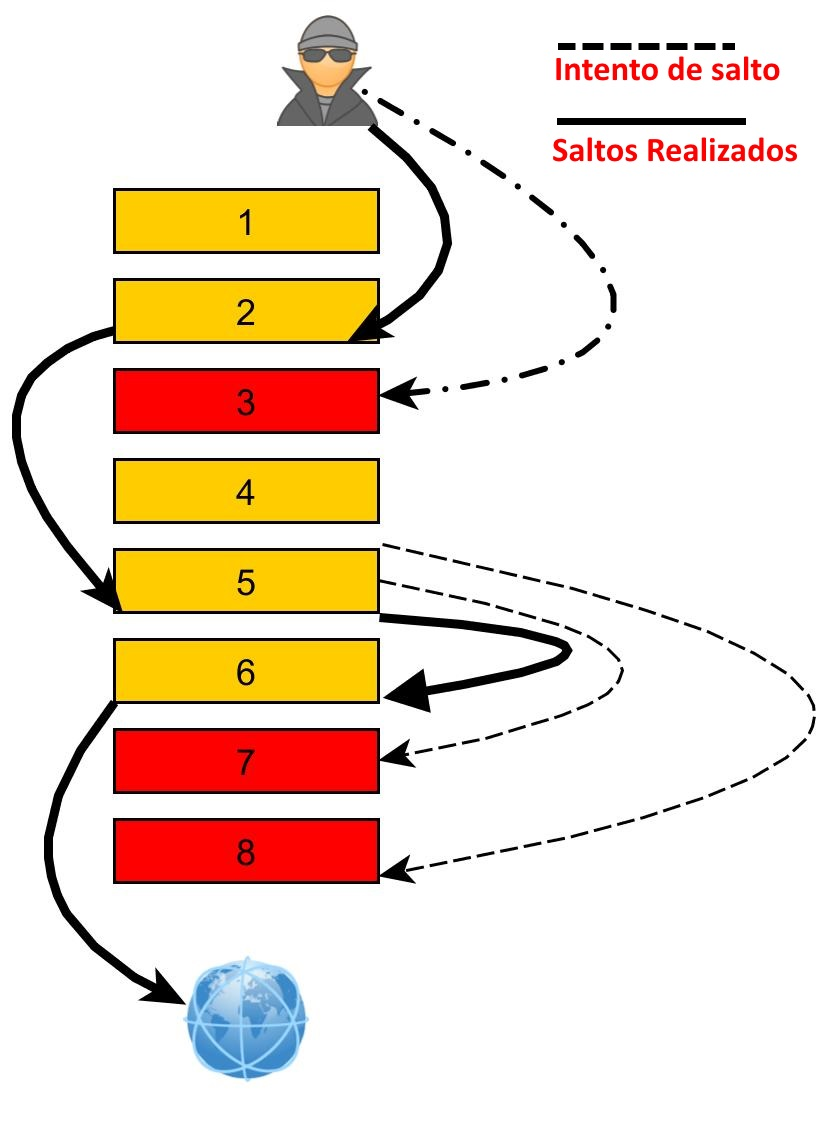
\includegraphics[scale=0.32]{ej1/unnamed0.jpg}
\end{figure}

Se ve claramente cómo cada vez que llega a un tablón prueba el tablón más lejano a su alcance, retrocediendo en caso de encontrar un tablón roto. 

En la siguiente sección formalizaremos esta idea y probaremos qué efectivamente los saltos mínimos se consiguen optando golosamente por el salto más lejano en cada momento.


\subsection{Justificaci\'on de correctitud}

A continuaci\'on presentamos un pseudoc\'odigo del algoritmo goloso empleado a fin de demostrar su correctitud.

\begin{algorithm}[H]
	 cantSaltos $\leftarrow$ 0 \\
     \While{no salí del puente}{
    	salto C tablones\\
        cantSaltos + 1 \\
        \While{no estoy en un tablón sano}{
        	retrocedoUno\\
            \If{volvíAlPrincipio}{no es posible cruzar\\}
         registroDóndeEstoy \\
         }
         }
         \caption{Pseudoc\'odigo para demostrar correctitud.Se asume que se recibe el puente con su cantidad de tablones y el salto máximo permitido}
\end{algorithm}

Este pseudocódigo no es más que una transcipción de la idea original en donde en cada iteración del ciclo principal se avanzan c tablones, se aumentan los saltos necesarios y si el tablón esta roto se retrocede o bien hasta encontrar un tablón sano o bien hasta volver al origen del salto en cuyo caso no habrá solución. Demostraremos entonces que este procedimiento efectivamente cumple con lo pedido.

Supongamos que \textbf{el problema tiene soluci\'on}, que \textbf{estamos en el tabl\'on $k$}, y queremos decidir a cu\'al de los tablones en el intervalo $(k..k+C+1]$ saltar para minimizar la cantidad de pasos en la que voy a cruzar el puente. 

Entonces, como la cantidad de tablones es finita y s\'olo \textbf{avanzamos hacia adelante}, deber\'ia haber \textbf{un tabl\'on \'optimo }que permita \textbf{minimizar la cantidad de saltos totales}.

Supongamos que decido saltar al tabl\'on $k+j_{1}$ pudiendo haber saltado al tabl\'on $k+j_{2}$, con $j_{1} < j_{2} \leq C$. En el siguiente paso, tambi\'en voy a querer saltar al tabl\'on que minimize la cantidad total de saltos que voy a dar desde $k+j_{1}$. Como asumimos que el problema tiene soluci\'on, \textbf{este tabl\'on seguro que existe}. Llam\'emoslo $t$, donde $t > k+C$ (pues de lo contario ya habr\'ia llegado a este tabl\'on en el paso anterior). 

Observemos entonces que este tabl\'on si es accesible desde el tabl\'on $k+j_{1}$ entonces tambi\'en lo es desde el tabl\'on $k+j_{2}$ pues $j_{1} < j_{2} $ pero, la rec\'iproca no vale siempre pues podr\'ia suceder que este tabl\'on $t$ cumpla que $k+j_{1}+C+1 < t \leq k+j_{2}+C+1 $ (i.e. no podr\'ia llegar a $t$ desde $k+j_{1}$ mientras que s\'i podr\'ia haberlo alcanzado si hubiera saltado a $k+j_{2}$). 

De esta manera, saltando siempre al tablón sano más lejano Luego, nuestro algoritmo cumple el invariante de que en cada paso, saltamos a un tabl\'on perteneciente al conjunto de tablones \'optimo (es decir, que minimiza la cantidad de pasos totales). 

Si el problema no tuviera soluci\'on, entonces seguro es porque hay alguna secuencia de tablones malos de longitud mayor o igual que C. Este caso lo contemplamos en el pseudoc\'odigo de m\'as arriba: si en alg\'un momento el sujeto salta los C tablones y despues retrocede esos mismos C tablones, entonces asumimos que el problema no tiene soluci\'on y finalizamos.

\subsection{Justificaci\'on cota de complejidad}

Adicionalmente a la resolución del problema, se nos solicitó que nuestro algoritmo se comportara linealmente en el tiempo respecto de la cantidad ($n$) de tablones del puente recibido como entrada (i.e. complejidad  $O(n)$ ). 

Como ya dijimos en secciones anteriores, el algoritmo hace que el individuo intente saltar la mayor cantidad de tablones posibles en funci\'on de su capacidad $c$ de salto y, si al intentar saltar esa cantidad de tablones se diera cuenta que va a caer en uno de los tablones rotos, el individuo deber\'ia ir retrocediendo uno a uno en los tablones anteriores al que pretend\'ia llegar hasta encontrar uno que no este roto, y saltar a ese. \\

Para mostrar que no hace falta más de $n$ iteraciones para recorrer el puente, vamos a mostrar que cada 2 iteraciones se avanzan al menos $c$ casilleros si hay solución (realizando $c$ veces el ciclo de retroceso) y que, entonces, la guarda del ciclo principal se reduce en $c$ cada 2 iteraciones. 

De esta manera, en cada iteración del ciclo principal, por cada vez que se ejecuta el subciclo de retroceso (tiempo constante $O(1)$), se descuenta una iteración de la guarda del ciclo principal, pudiendo decirse entonces que el algoritmo toma tiempo lineal (en la cantidad de tablones). 

Veamos que en la \textbf{iteración $i$}si el sujeto \textbf{estaba en el tabl\'on $k$} es porque \textbf{retrocedió $j$ tablones en el paso $i-1$}( $j<c$, ya que si $j=c$ entonces no hay solución); entre el tabl\'on $k$ y el $k+j$ no hay ning\'un tabl\'on sano. De esta forma, en el paso $i+1$ el sujeto tendr\'a que retroceder no m\'as de $k+c-k-j = c-j$ tablones luego de saltar, ya que los $j$ tablones después de k no están sanos. 

Esto implica que entre el paso $i-1$ y el paso $i$, en el peor caso el sujeto no recorreria m\'as de $c-j+j=c$ tablones, habiendo avanzado un total de $c-j+k+j+1-k-1 = c$ tablones.

As\'i vemos entonces que se cumple que en el peor caso cada 2 iteraciones se avanzan $c$ tablones que son descontados de la guarda del ciclo principal. De esta forma, como dicho ciclo contiene asignaciones de tiempo constante y el subciclo de retroceso también, el recorrido que hace el algoritmo es lineal ya que las iteraciones constantes que realiza en el subciclo, las descuenta del ciclo más grande.

\begin{lstlisting}[caption=Fragmento de código c++ encargado del ciclo principal y el subciclo de retroceso]
	  actual = 0; cantPasos = 0;	

	  while(actual <= n) {			// hasta haber cruzado el puente, hago..
		
			temp = 0; actual += c; // asinaciones O(1)
		
			while(temp < c && puente[actual] == 1) {	// retrocedo lo necesario	
														
			    actual--; //descuento iteraciones del ciclo grande O(1)
			    temp++;
		    }
		    if(temp == c) {cout << "no" << endl; break; }	// sin solucion. No analizamos complejidad de I/O
		
	        res[cantPasos] = actual; cantPasos++;			// registro el nuevo salto
	  }
\end{lstlisting}


\subsection{Testeos de complejidad}
En la presente sección analizaremos experimentalmente la complejidad temporal del algoritmo propuesto para la resolución del problema planteado.

\subsubsection{Medición de tiempos y generación de entradas}
Para medir los tiempos usamos la biblioteca \textit{time.h}. Medimos solamente nuestra implementación (el tiempo empleado por el ciclo principal) sin contar las operaciones de entrada/salida.  

Para generar entradas pseudo aleatorias utilizamos un script que dado un $n$ ubicaba tablones rotos o sanos con igual probabilidad generando asi un archivo de entrada para este algoritmo.

\subsubsection{Gráficos}

Presentaremos 2 gráficos. 

El primero consiste en la comparación para tiempos de ejecución en 3 casos. Una instancia aleatoria con $c$ muy pequeño (en relación a $n$), otra con c en función de n ($\frac{n}{10000}$) y finalmente la instancia de peor caso de nuestro algoritmo que notamos en la demostración de complejidad (con sólo un tablón sano cada $\frac{c+1}{2}$ rotos) con $c=25$.

El segundo gráfico tendrá una comparación de los tiempos para instancias aleatorias modificando el c.

\begin{figure}[H]
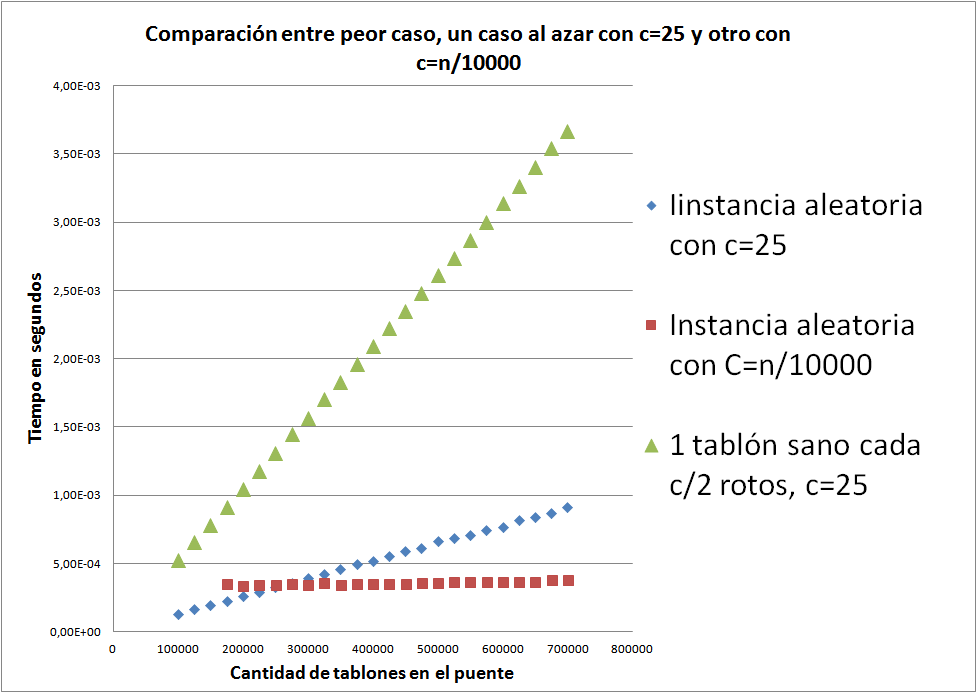
\includegraphics[scale=0.5]{ej1/graph_1.png}
\caption{Gráfico de tiempos para la ejecución de 3 instancias distintas. Peor caso e instancia aleatoria con c fijo y c dependiente de n}
\end{figure}

\begin{figure}[H]
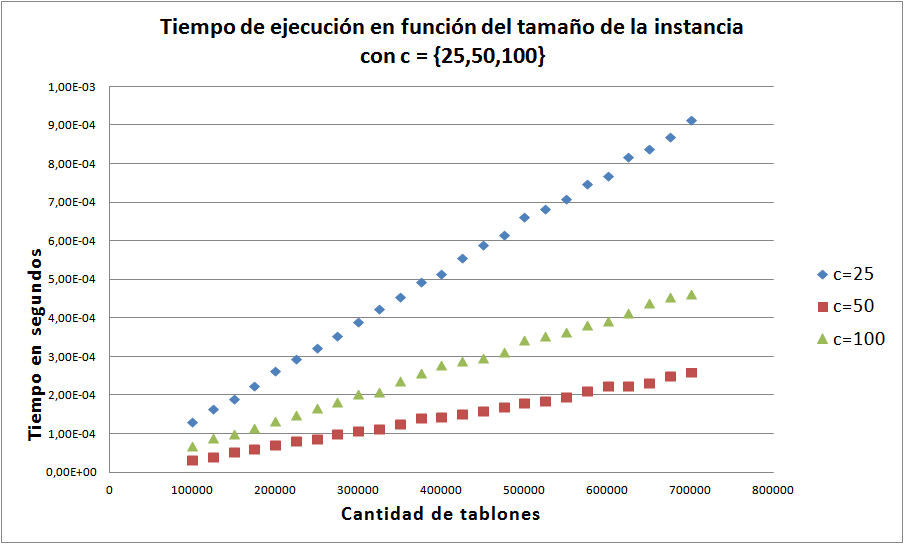
\includegraphics[scale=0.5]{ej1/graph_2.png}
\caption{Gráfico de tiempos para la ejecución de 3 instancias distintas. ($c=25$, $c=50$, $c=100$)}
\end{figure}

De la observación de los gráficos podemos notar el comportamiento lineal esperado de nuestro algoritmo para todas las instancias.

En el primer gráfico comprobamos empíricamente la existencia del peor caso que dedujimos de la demostración de complejidad. Este caso es considerablemente peor al de una instancia  aleatoria con el mismo c. A su vez notamos que, si el c respeta una misma proporción con el tamaño de la entrada, el algoritmo se comporta de forma más o menos constante ya que la cantidad de saltos presumiblemente será similar en todas las instancias (a lo sumo se modificará en 1 salto).
 
En el segundo gráfico vemos el impacto del c en el tiempo de ejecución para las mismas instancias aleatorias. A medida que se le permite saltar más tablones por vez, el algoritmo ejecuta cada vez más rápido.

Finalmente vale aclarar que no observamos distintas formas de distribuir tablones a lo largo del puente porque lo que realmente es significativo es si el tablón más lejano después de cada salto está roto o no y cuántos rotos seguidos hay antes de ese, siendo justamente el peor caso en cual hay exactamente la mitad del salto máximo de tablones.

Podemos entonces decir que este algoritmo se ve afectado en su tiempo por la cantidad máxima de tablones permitidos por salto y por la distribución de los tablones sobre el puente


\subsection{Adicionales}

\textbf{XXXXXXXXXXXXXXXXXXXXXXXXXXXXXXXXXXXXXXXXXXXXXXXXXXXXXXX}
\clearpage